\documentclass[compsoc,draftclsnofoot,onecolumn,10pt]{IEEEtran}
\usepackage[utf8]{inputenc}
\usepackage{color}
\usepackage{url}

\usepackage{enumitem}

\usepackage[letterpaper, margin=.75in]{geometry}
\usepackage{hyperref}
\usepackage{listings}

\usepackage[dvipsnames]{xcolor}
\usepackage{pgfgantt}
\newcommand*{\SignatureAndDate}[1]{
    \par\noindent\makebox[2.5in]{\hrulefill} \hfill\makebox[2.0in]{\hrulefill}
    \newline\noindent\makebox[2.5in][l]{#1}  \hfill\makebox[2.0in][l]{Date}
}
\usepackage{etoolbox}
\patchcmd{\thebibliography}{\section*}{\subsection}{}{}
\patchcmd{\thebibliography}{\addcontentsline{toc}{section}{\refname}}{}{}{}

\usepackage{graphicx}

\definecolor{dkgreen}{rgb}{0,0.6,0}
\definecolor{gray}{rgb}{0.5,0.5,0.5}
\definecolor{mauve}{rgb}{0.58,0,0.82}

\renewcommand{\lstlistingname}{Code Example} % a listing caption title.

\lstset{
	frame=single,
	language=C,
	columns=flexible,
	numbers=left,
	numbersep=5pt,
	numberstyle=\tiny\color{gray},
	keywordstyle=\color{blue},
	commentstyle=\color{dkgreen},
	stringstyle=\color{mauve},
	breaklines=true,
	breakatwhitespace=true,
	tabsize=4,
	captionpos=b
}

\def\name{Cierra Shawe, Daniel Stoyer, Tao Chen}

%% The following metadata will show up in the PDF properties
\hypersetup{
	colorlinks = false,
	urlcolor = black,
	pdfauthor = {\name},
	pdfkeywords = {SRS requirements, Fall 2016},
	pdftitle = {SRS requirements},
	pdfsubject = {Requirement document for ARCt},
	pdfpagemode = UseNone
}

\def\myversion{1.0 }
\date{}
%
%\usepackage{titlesec}
%
%\usepackage{hyperref}

\parindent = 0.0 in
\parskip = 0.1 in

\setcounter{secnumdepth}{5}

\begin{document}

\begin{titlepage}
\title{
Software Requirements Specification\\
\LARGE
ARC - Autonomous RC\\
Senior Capstone Project\\
Oregon State University\\
Fall 2016
}
\author{Tao Chen, Cierra Shawe, Daniel Stoyer}
\maketitle
\begin{center}
	Version 1.0\\
	\today
\end{center}

\vspace{1cm}
	
\SignatureAndDate{D. Kevin McGrath} \newline\newline
\SignatureAndDate{Tao Chen}\newline\newline
\SignatureAndDate{Cierra Shawe}\newline\newline
\SignatureAndDate{Daniel Stoyer}\newline\newline
    

\thispagestyle{empty} % gets rid of the "0" page number.
	
\end{titlepage}

\tableofcontents

\newpage

\section{Introduction} % Section 1; Cierra, Done
This document aims to provide an overview and list of requirements for group 44, Autonomous RC (ARC). 
This section provides a purpose and scope description, list of abbreviations and acronyms, and an overview of everything included in this SRS document. 
As this is a research project, some of the sections within the document may not apply to the project. 


\subsection{Purpose} % Cierra, Done
A detailed description of the requirements for the "Autonomous RC System" or ARCS will be provided within this document. 
System constraints, interface decisions, and interactions with other external applications and hardware will also be explained. 
This document is primarily intended to be a customer proposal for approval and a development team reference for the first version of the system.

\subsection{Scope} % Cierra, Done
ARCS is a software-hardware interface designed to retrofit RC cars for autonomous operation, using commodity hardware. 
The software and hardware specifications should be available free to download and modify at the users will. \par
Users should be able to purchase and install the specified hardware from major online retailers such as Amazon.com or hobby sites such as Sparkfun.com.
Once the vehicle is assembled, it should be able to autonomously navigate to a given destination using GPS, or a within pre-defined boundaries, such as a room.  
Control software will need to be loaded onto the main processing unit and any other control hardware needed. 
Other software required will be a control panel to monitor the vehicle and determine it's behavior, such as navigating to a point, or on a track. 

Hardware that we expect to need:
\begin{itemize} 
\item Base station that includes a transceiver
\item An RC car with servo steering and DC motors
\item Main processing unit (a computer)
\item Transceiver to send and receive information on the car
\item Controller to send signals to sensors and actuation devices (motors, servos, etc...) 
\item Vision system to aide in obstacle avoidance
\item GPS unit to aide in navigation
\end{itemize}

ARCS will be expected to be able to receive input from a user base station, and react
within the environment based on a destination or path that the system receives. It should also
be able to navigate to the destination without user intervention, as fast as possible. \par

\subsection{Definitions, Acronyms, and Abbreviations} % Tao, in progress
\begin{enumerate}
	\item \textbf{IMUs:} Inertial measurement unit. Used to measure acceleration, angular acceleration, and orientation of the vehicle.
	\item \textbf{Operator/User:} The person who is giving commands such as destination to the system.
	\item \textbf{Protocol:} Defines the data format to be transferred.
	\item \textbf{Telemetry Data:} Data that contains the status information of the vehicle, such as speed, temperature, location, battery, etc.
	\item \textbf{Emergency:} Emergencies include, but are not limited to: 
	\begin{itemize}
		\item The vehicle drifts off course significantly.
		\item Vehicle flips upside down.
		\item On-board components fall off.
	\end{itemize}
	\item \textbf{Visual Unit:} Visual components that provide image streams to the main processing unit. 
	The primary computer will extract information from the images, such as road condition, obstacles, and depth. 
	\item \textbf{Actuators:} Motors and servos.
	\item \textbf{Initialization:} From the system perspective, the initialization process will include self-checking and sensor calibration. 
	From the user's perspective, it contains making sure all the hardware is attached, battery is at least 80\% full, and giving the system a destination. 
	\item \textbf{Success:} The vehicle successfully navigates itself to the destination.
	\item \textbf{ARC:} Autonomous Remote Controlled is our team name
	\item \textbf{ARCS:} ARC System, which refers to both hardware and software components built for the project.
	\item \textbf{RC:} Remote Controlled
	\item \textbf{AV:} Autonomous Vehicle
	\item \textbf{Main Processing Unit:} The unit which handles all high level decisions and input processing. 
	\item \textbf{Stakeholder:} Any user that will operate ARCS.
	\item \textbf{Companion Computer:} The computer on board the RC vehicle that performs heavy computation, such as image analysis.
	\item \textbf{Ground Station:} The remote computer that sends user commands to the vehicle and receives telemetry from the vehicle.
	\item \textbf{Graphical User Interface (GUI):} a way to visually interact with the ARC environment using mouse and keyboard.
	\item \textbf{Command Line Interface (CLI):} a text-based interface that allows entering commands from a prompt, usually executed from within a terminal or shell.
	\item \textbf{Mission:} The total operations of the vehicle, as commanded by the user. For example, a user tells the vehicle to go to a point at a certain speed, that is the mission for the vehicle.
\end{enumerate}

% References
\bibliographystyle{IEEEtran}
\bibliography{srs}

\subsection{Overview} % Cierra, Done 
The remainder of this document includes three sections and the appendixes. \par
Section two provides an overview of system functions and intersystem interaction. 
System constraints and assumptions are also addressed. \par
Section three provides the requirement specification in detailed terms and system interface descriptions. 
Different specification techniques are used in order to specify requirements for different audiences. \par
Section four priorities requirements and includes motivation for the chose prioritization and discusses why other methods were not chosen. \par
Appendixes at the end of the document include results of the requirement prioritization and a release plan based on the requirements. \cite{IEEE830}

%%%%%%%%%%%%%%
\section{Overall Description} % Section 2; Cierra, Done
This section will explain the system in its context to create a better understanding of how the system interacts with other systems.
In addition, basic functionality will be introduced and addressed. 
Stakeholders will be defined and functionality for each type of stakeholder will be addressed. 
Lastly, constraints and assumptions for the system will be presented. 

%%%%%%%%%%%%%%%%
\subsection{Product Perspective} % Cierra, kinda done for now
ARCS will be designed to integrate into an RC car using commodity hardware, and open to anyone who is interested in using it. This 
makes ARCS a component of a larger system, namely the RC car. \par
ARCS will consist of three parts: 
\begin{enumerate}
	\item Base-station used for user interaction
	\item Hardware attached to RC car to be able to connect to base-station and 
		operate the vehicle
	\item Software implementation for control and communication between hardware and software
\end{enumerate}
In order for the user to interact with the vehicle, commands will be sent via some form
of receiver to the car. This will need to be done via a base-station that has software able of
providing a way to communicate with the receiver, which then transmits data to the receiver on 
the car, which is then handled by the on-board computer. 
The control flow is described in figure 1. \\

%%% THIS IS FOR DRAWING THE BLOCK DIAGRAM %%%git 
\begin{figure}
  \centering
 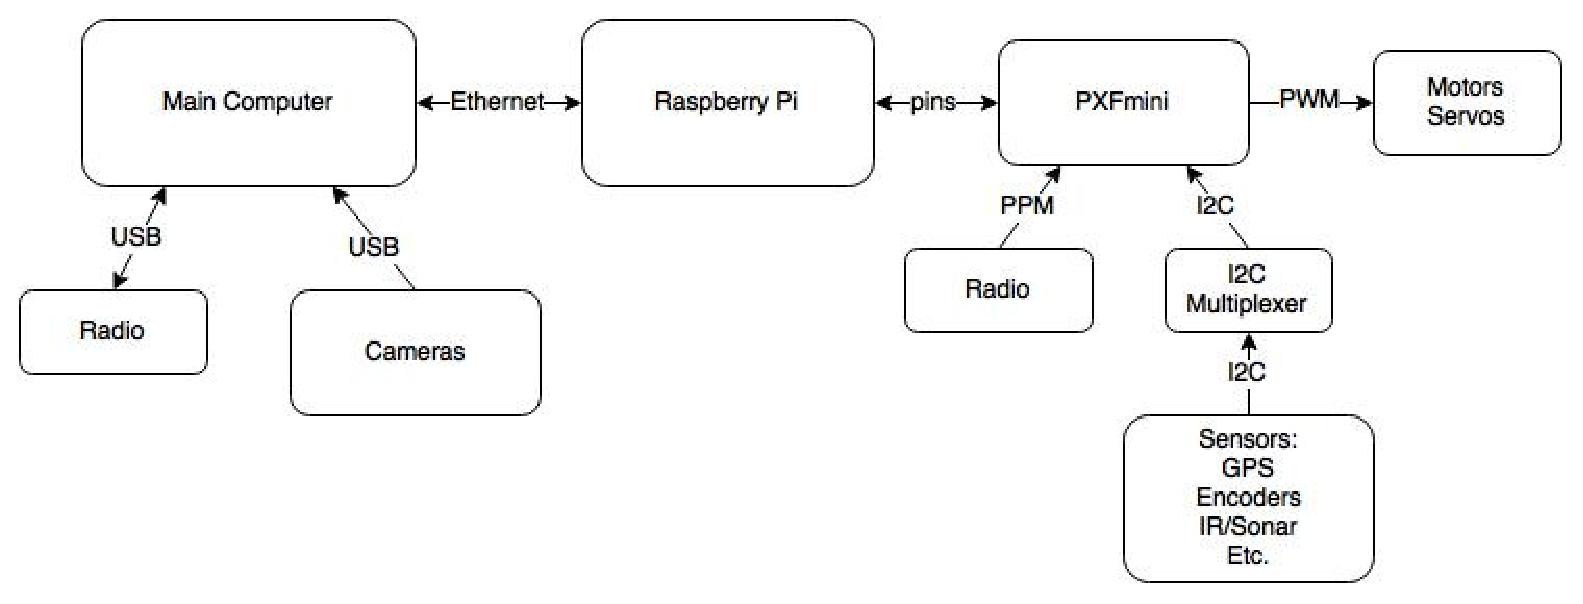
\includegraphics[width=\textwidth]{Block_Diagram_1_.eps}
  \caption{Block diagram of hardware flow}
\end{figure}


\subsubsection{System interfaces} %Tao, finished
There are a total of 5 system interfaces where the system can communicate with 
the outside world.
\begin{enumerate}
	\item Sensors: Sensors will have a two-way communication with a secondary computer unit, where filtering and smoothing will happen before reliable data will be passed to the main processing unit. 
	The programs that reside in the secondary unit will utilize various methods to generate reliable results based on the raw data. 
	At start-up, there will be a script executed by the system to correctly configure and calibrate each sensor. 
	Sensors may include: battery monitor, temperature sensor, GPS, encoders, IMUs, and any other sensors that are needed for autonomous operation.
	\item Radio: This is the portal of the system where operator/user can monitor the status of the vehicle. 
	Different protocols will be implemented for telemetry data, which will be displayed to the operator/user. 
	This portal also allows operator/user to take control over the computer in case of emergencies. 
	\item Visual unit: This is the interface where the visual unit can pass streams of images to the system.
	\item Actuator: The system issues commands to the motors and servos via this interface. 
	\item User interface: This interface is a different interface than the radio interface even though they both allow humans to interact with the system. 
	The user interface will be disable after the vehicle starts maneuvering. 
	This interface allows user to input operation modes and desired destinations into the system.
\end{enumerate}

\subsubsection{User interfaces} %Tao, finished
The user interface will be a graphical user interface (GUI) that can be interacted with by a user. 
Anyone who knows how to operate a mouse or touch screen will be al. 
A map makes it easier for users to pin point destinations and view the current location of the vehicle. 
An error messages will be generated the vehicle and the station exceeds the maximum radio range, or the vehicle is low on battery.\par
With proper training (in less than 30 minutes), one can understand all the indicators of the system to know the status of the vehicle.\par
The GUI is a single window/page arrangement. 
A large portion of the window is dedicated to the map. 
A section of the GUI will be used to display telemetry data. 
Error messages will cover at least 10\% of the screen in order to alert the user of an issue.

\subsubsection{Hardware Interfaces} % Cierra
Two main hardware interfaces currently exist within ARCS. 
\begin{enumerate}
	\item Vision processing
	\item Telemetry collection and actuator control
\end{enumerate}

Vision processing, from either a stereoscopic or depth camera, will be interfaced through 
an i5 or better processor from an on board computer using a control board, which will be used as an interface between a 
computer that is doing high level computations, the servos, motors, and other telemetry 
devices. 

Telemetry collection and actuator control will be handled by a PXFmini and interfaced through a board with a 40pin connector, such as the Raspberry Pi. This abstracts a lot of control onto the PXFmini. 

\subsubsection{Software Interfaces} % Dan
\begin{itemize}
	
	\item We require three operating systems. One for a remote PC for user input, one
	for the primary computer for on-car data analysis, and one for the secondary
	computer for on-car control.
	
	\item We require a user interface to be able to give the car destination commands. 
	
	\item We require software that takes input from hardware, such as video cameras,
	and analyze the data 
	
	\item Sensor analysis software needs to be able to read data from sensors, such IMUs, and generate usable information to pass on to 
	
	\item Path finding software needs to be able to integrate and analyze data from mapping and localization software products and determine a path to follow in real time.
	
	\item The primary and secondary computers will need to talk with one another. The
	primary computer will need to receive data from the secondary computer,
	analyze the data and send corresponding commands back to the secondary
	computer. The secondary computer will need to receive commands from the
	primary computer, and send data to the primary computer.
	
	\item A software interface will required on the secondary computer to convert
	commands received from the primary computer to instructions usable by
	pre-existing RC car on-board controller.
	
	\item We will require separate interfaces between the secondary computer and the
	visual/spacial sensors, GPS, speed sensor, and the IMU. 
	
\end{itemize}


\subsubsection{Communications Interfaces} % Dan
%This should specify the various interfaces to communications such as local
%network protocols, etc.
\begin{itemize}
	\item Radio communication will required to be able to send commands to the car and
	to be able to receive feedback from the car. The radio frequency will be in 27
	MHz or 49 MHz range. We need software that allows us to send and receive radio
	signals to and from the car. 
	
	\item LAN communication will be used to transmit data between the on-car computers.
	Existing network protocols will be utilized to perform the transmissions.
	
	\item A software interface will be required to send the commands from the
	secondary computer to the pre-existing RC car on-board controller.
	
\end{itemize}


\subsubsection{Memory constraints} %Tao, done
%This should specify any applicable characteristics and limits on primary and
%secondary memory.
Since we are unsure of what hardware will be used, we are not able to set any 
constraints on the memory requirements that the system has to meet. 

\subsubsection{Operations} %Tao
In most cases, operations of the system will be isolated from the user/operator,
excluding emergencies and initialization.  
%This should specify the normal and special operations required by the user such as
\begin{enumerate}
	\item At initialization, user/operator has to thoroughly check the body of the
	vehicle, making user that all components are firmly attached as well as the 
	battery level is at least 80\%;
	\item Destination will be given by the user at the station during initialization;
	\item User is allowed to take over control from the system in case of emergencies
	via the remote control;
	\item User/operator is responsible for monitoring the status of the system, such as 
	battery level, speed, location, distance, radio signal strength, pre-planned path, 
	etc.
\end{enumerate}
%This could the extension of the user interface section.
%This is sometimes specified as part of the User Interfaces section.

\subsubsection{Site Adaptation Requirements}
For research and prototype purposes, no site adaptation requirements are relevant. 

\subsection{Product Functions} %Tao, finished
This system utilizes resources from more than one computer and controls multiple actuators. 
The system is designed to minimize user interference during operations, however, monitoring is required.
Maintainability of the system is not considered to be user-oriented, which means a user/operator should not be worried about maintaining the system. 
The system will be made available publicly (open source), however, only users with extensive robotics experience should attempt at modifying the system outside of the given parameters.


\subsection{User Characteristics} % Cierra
Our system should be able to be built and operated by a user with at least two 
years of university engineering coursework and one two years, a user with over 
five years of technical experience through work in either an electrical or software 
industry, and a RC hobbyist with over five years of experience. 

\subsection{Constraints} % Tao, finished
As this is a research project, constraints may rapidly change or new constraints may be retroactively added to better address problems found or the needs of the system. \par
Current constraints for the project include: 
\begin{enumerate}
	\item Real time image processing will limit the vehicle's ability to maneuver through obstacles. 
	\item Telemetry data displayed to the user will be slightly delayed due to long distance. 
	No solutions to this issue are currently available.
	\item The vehicle's natural structure will inevitably cause more uncertainty on predictions, which requires the use of more complicated algorithms versus what is required for ideal conditions.
	\item Hardware may fall off during operation which will force the system to halt. 
	All components must be securely fastened and adequately protected in the case of an emergency.  
	\item Telemetry data transfer are limited to radio during outdoor operations.
	\item The success rate are set to 80\% and above.
	\item For research purpose only, the vehicle will only be required to navigate around static objects in an environment. 
	This is to reduce the complexity of the initial system. 
\end{enumerate}

\subsection{Assumptions and Dependencies}
As a research project, the main assumption is currently this is possible. 

\subsection{Apportionment of Requirements} % Dan, in progress
See next page.
%This subsection of the SRS should identify requirements that may be delayed
%until future versions of the system.


%%%%%%%%%% How to use these Gantt Charts %%%%%%%%%%
%%% IMPORTANT!!! %%%
% Within the \ganttchart[]{} code, ONLY adjust dates
%
% Each Gantt chart has an area preceding it to adjust values.
%
% When adding a group or task, use the existing code in the SRS section as a 
% template.
%
% The overall progress for a group is tracked by getting the average of all the 
% subtasks. So, if you add a subtask, be sure to add the count variable to the
% overall average computation and increase the denominator by one
% Example progress average:
%
% \newcount\srsprogress
% \srsprogress=\the\numexpr(
% 	  \introprog 
% 	+ \overalldescprog 
% 	+ \specificreqprog 
% 	+ \othernonfunreqprog 
% 	+ \otherreqprog
% 	+ \indexprog 
% 	+ \appendixprog
% 	)/7 % divided by number of subtasks
%%%%%%%%%%%%%%%%%%%%%%%%%%%%%%%%%%%%%%%%%%%%%%%%%%%


%%%%% Fall Term Chart Oct 14 - Dec. 09 %%%%%%%

%%%%%%%%%%%%%%%%%%%%%%%%%%%%%%%%%%%%%%%%%%%%%%%%%%%
% Set progress and dates for groups and tasks here.
%%%% Term Date Range %%%%
\newcommand{\fallstart}{2016-10-14}
\newcommand{\fallend}{2016-12-09}

%%%% SRS (Due: Oct 28) %%%%

%Introduction
\newcount\introprog
\introprog=100

% Overall Description
\newcount\overalldescprog
\overalldescprog=100

% Specific Requirements
\newcount\specificreqprog
\specificreqprog=100

% Other Non-Functional Requirements
\newcount\othernonfunreqprog
\othernonfunreqprog=100

% Other Requirements
\newcount\otherreqprog
\otherreqprog=100

% Index
\newcount\indexprog
\indexprog=100

% Apppendix
\newcount\appendixprog
\appendixprog=100

% Overall SRS progress

% NOTE
\newcount\srsprogress
\srsprogress=\the\numexpr(
  \introprog 
+ \overalldescprog 
+ \specificreqprog 
+ \othernonfunreqprog 
+ \otherreqprog
+ \indexprog 
+ \appendixprog
)/7
%%%%%%%%%%%%%%%%%%%%%%

%%%% Technology Review (Due: Nov. 04) %%%%
\newcount\techprogress
\techprogress=100
%%%%%%%%%%%%%%%%%%%%%%

%%%% Design Document (Due: Nov. 23) %%%%
\newcount\designprogress
\designprogress=100
%%%%%%%%%%%%%%%%%%%%%%

%%%% Fall Progress Report (Due: Dec. 09) %%%%
\newcount\fprogress
\fprogress=100
%%%%%%%%%%%%%%%%%%%%%%

%%%%%%%%%%%%%%%%%%%%%%%%%%%%%%%%%%%%%%%%%%%%%%%%%
\begin{figure}[h]
	\caption{ARC Fall Schedule Gantt Chart}	
	\begin{ganttchart}[
		y unit title=0.4cm,
		y unit chart=0.5cm,
		x unit=0.2665cm,
		vgrid,
		%	time slot format=isodate-yearmonth,
		time slot format=isodate,
		%	compress calendar,
		title/.append style={fill=RoyalBlue!50!black},
		title label font=\sffamily\bfseries\color{white},
		title label node/.append style={below=-1.6ex},
		title left shift=.05,
		title right shift=-.05,
		title height=1,
		bar/.append style={draw=none, fill=OliveGreen!75},
		bar height=.6,
		bar label font=\normalsize\color{RawSienna},
		group/.append style={draw=none, fill=MidnightBlue},
		group incomplete/.append style={fill=YellowOrange},
		group right shift=0,
		group top shift=.6,
		group height=.3,
		group peaks height=.2,
		bar incomplete/.append style={fill=Maroon}
		]{\fallstart}{\fallend}
		
		\ganttset{
			calendar week text={
				\pgfcalendarmonthshortname{\startmonth}~\startday
			}
		}
		\gantttitle{Fall 2016}{57}\\
		\gantttitlecalendar{week} \\
		\ganttset{progress label text={}, link/.style={black!63, -to}}
		
		%%%% SRS (Due: Oct 28) %%%%
		\ganttgroup[progress={\srsprogress}]{Requirements Document}{2016-10-14}{2016-10-28} \\
		\ganttbar[progress={\introprog}]{Introduction}{2016-10-14}{2016-10-28} \\
		\ganttbar[progress={\overalldescprog}]{Overall Description}{2016-10-14}{2016-10-28} \\
		\ganttbar[progress={\specificreqprog}]{Specific Requirements}{2016-10-14}{2016-10-28} \\
		\ganttbar[progress={\othernonfunreqprog}]{Other Non-Functional Req.}{2016-10-14}{2016-10-28} \\
		\ganttbar[progress={\otherreqprog}]{Other Req.}{2016-10-14}{2016-10-28} \\
		\ganttbar[progress={\indexprog}]{Index}{2016-10-14}{2016-10-28} \\
		\ganttbar[progress={\appendixprog}]{Appendix}{2016-10-14}{2016-10-28} \\
		
		
		%%%% Technology Review (Due: Nov. 04) %%%%
		\ganttgroup[progress={\techprogress}]{Tech Review}{2016-10-29}{2016-11-04} \\
		
		%%%% Design Document (Due: Nov. 23) %%%%
		\ganttgroup[progress={\designprogress}]{Design Doc}{2016-11-05}{2016-11-23} \\
		
		%%%% Fall Progress Report (Due: Dec. 09) %%%%
		\ganttgroup[progress={\fprogress}]{Fall Report}{2016-11-24}{2016-12-09} \\
		
		%	\ganttset{link/.style={OliveGreen}}
	\end{ganttchart}
\end{figure}

%%%%% Winter Term Chart JAN 09 - MAR 24 %%%%%

%%%%%%%%%%%%%%%%%%%%%%%%%%%%%%%%%%%%%%%%%%%%%%%%%%%
%%%% Term Date Range %%%%
\newcommand{\winterstart}{2017-01-09}
\newcommand{\winterend}{2017-03-24}

% Set progress and dates for groups and tasks here.

%%%% Alpha level release (with demo) (Due: Feb. 24, 2017) %%%%
\newcount\alphaprogress
\alphaprogress=75

%%%% Beta level release (with demo) (Due: Mar. 24, 2017) %%%%
\newcount\betaprogress
\betaprogress=0

%%%% Winter progress report (Due: Mar. 24, 2017) %%%%
\newcount\wprogress
\wprogress=0
%
%
%
%
%%%%%%%%%%%%%%%%%%%%%%%%%%%%%%%%%%%%%%%%%%%%%%%%%%%
\begin{figure}[h]
	\caption{ARC Winter Schedule Gantt Chart}
	\begin{ganttchart}[
		y unit title=0.4cm,
		y unit chart=0.5cm,
		x unit=0.227cm,
		vgrid,
		%	time slot format=isodate-yearmonth,
		time slot format=isodate,
		%	compress calendar,
		title/.append style={draw=none, fill=RoyalBlue!50!black},
		title label font=\sffamily\bfseries\color{white},
		title label node/.append style={below=-1.6ex},
		title left shift=.05,
		title right shift=-.05,
		title height=1,
		bar/.append style={draw=none, fill=OliveGreen!75},
		bar height=.6,
		bar label font=\normalsize\color{RawSienna},
		group/.append style={draw=none, fill=MidnightBlue},
		group incomplete/.append style={fill=YellowOrange},
		group right shift=0,
		group top shift=.6,
		group height=.3,
		group peaks height=.2,
		bar incomplete/.append style={fill=Maroon}
		]{\winterstart}{\winterend}
		
		\ganttset{
			calendar week text={
				\pgfcalendarmonthshortname{\startmonth}~\startday
			}
		}
		\gantttitle{Winter 2017}{75}\\
		\gantttitlecalendar{week} \\
		\ganttset{progress label text={}, link/.style={black!63, -to}}
		
		%%%% Alpha level release (with demo) (Due: Feb. 24, 2017) %%%%
		\ganttgroup[progress={\alphaprogress}]{Alpha Release}{2017-01-09}{2017-02-24} \\
		
		%%%% Beta level release (with demo) (Due: Mar. 24, 2017) %%%%
		\ganttgroup[progress={\betaprogress}]{Beta Release}{2017-02-25}{2017-03-24} \\
		
		%%%% Winter progress report (Due: Mar. 24, 2017) %%%%
		\ganttgroup[progress={\wprogress}]{Winter Report}{2017-02-25}{2017-03-24} \\
		
		%	\ganttset{link/.style={OliveGreen}}
	\end{ganttchart}
\end{figure}

%%%%%% End Winter Term %%%%%

%%%%%% Spring Term Chart APR 3 - JUN 16 %%%%%

%%%%%%%%%%%%%%%%%%%%%%%%%%%%%%%%%%%%%%%%%%%%%%%%%%%%%%%
%%%% Term Date Range %%%%
\newcommand{\springstart}{2017-04-03}
\newcommand{\springend}{2017-06-16}
%	% Set progress and dates for groups and tasks here.


%%%% 1.0 level release (Due: May 15, 2017) %%%%
\newcount\releaseprogress
\releaseprogress=0

%%%% Engineering Expo (Due: May 19) %%%%
\newcount\expoprogress
\expoprogress=0

%%%% Final Report (Due: June 16) %%%%
\newcount\finalrepprogress
\finalrepprogress=0
%
%
%
%%%%%%%%%%%%%%%%%%%%%%%%%%%%%%%%%%%%%%%%%%%%%%%%%%%%%%%
\begin{figure}[h]
	\caption{ARC Spring Schedule Gantt Chart}	
	\begin{ganttchart}[
		y unit title=0.4cm,
		y unit chart=0.5cm,
		x unit=0.231cm,
		vgrid,
		%	time slot format=isodate-yearmonth,
		time slot format=isodate,
		%	compress calendar,
		title/.append style={draw=none, fill=RoyalBlue!50!black},
		title label font=\sffamily\bfseries\color{white},
		title label node/.append style={below=-1.6ex},
		title left shift=.05,
		title right shift=-.05,
		title height=1,
		bar/.append style={draw=none, fill=OliveGreen!75},
		bar height=.6,
		bar label font=\normalsize\color{RawSienna},
		group/.append style={draw=none, fill=MidnightBlue},
		group incomplete/.append style={fill=YellowOrange},
		group right shift=0,
		group top shift=.6,
		group height=.3,
		group peaks height=.2,
		bar incomplete/.append style={fill=Maroon}
		]{\springstart}{\springend}
		
		\ganttset{
			calendar week text={
				\pgfcalendarmonthshortname{\startmonth}~\startday
			}
		}
		\gantttitle{Spring 2017}{75}\\
		\gantttitlecalendar{week} \\
		\ganttset{progress label text={}, link/.style={black!63, -to}}
		
		%%%% 1.0 level release (Due: May 15, 2017) %%%%
		\ganttgroup[progress={\releaseprogress}]{1.0 Release}{2017-04-03}{2017-05-15} \\
		
		%%%% Engineering Expo (Due: May 19) %%%%
		\ganttgroup[progress={\expoprogress}]{Spring Expo}{2017-05-16}{2017-05-19} \\
		
		%%%% Winter progress report (Due: Mar. 24, 2017) %%%%
		\ganttgroup[progress={\finalrepprogress}]{Final Report}{2017-05-20}{2017-06-16} \\
		
		%	\ganttset{link/.style={OliveGreen}}
	\end{ganttchart}
\end{figure}

%%%%%% End Spring Term %%%%%


\section{Specific Requirements} % Section 3
This section describes the hardware, software, and performance requirements
necessary for the ARC system to function. It lays out requirements for
input and output of the system through interfaces. It also covers the major
systems features and functional requirements for those features.

\subsection{External interface requirements}
This section describes all of the interfaces required for input to and output
from the ARC system.
	\subsubsection{User interfaces}
	There should be a remote station (commonly referred to as a ground station) where all information about the vehicle can be seen.
	The ground station should allow user control of the vehicle including setting way-points, adjusting parameters for vehicle behavior, and direct control over vehicle movement.
	
	\subsubsection{Hardware interfaces}
	There should be hardware interfaces for manual control of the vehicle. 
	This interface should be able to override software control so that users can safely commandeer control of the vehicle from the autopilot. 
	Other hardware interfaces should be between a network interface between the autopilot and the companion computer on the vehicle.
	There should also be a hardware interface between the autopilot and the vehicle control system.
	We will use existing protocols for communication between the autopilot and the companion computer and the vehicle.

	\subsubsection{Software interfaces}
	There should be software interfaces between the user interfaces and the hardware interfaces. These interfaces will be handled by the operating system on both the ground station and the companion computer.

\subsection{System features}
Describes what the ARC system can be expected to do in terms of its major features.

\subsubsection{System Feature: Image Analysis}
	
	\paragraph{Functional requirement image analysis 1}
		\begin{enumerate}
			\item ID: FR-IA1
			\item Title: Fast Image Processing.
			\item Description: Image analysis needs to be at a rate of around 15 or more frames per second.
			\item Rationale: In order for the vehicle to move fast, images will need to be acquired and processed very fast.
			\item Dependencies: N/A
			\item Completion Metric: Frames per second being processed will be displayed to the user. 
		\end{enumerate}	

	\paragraph{Functional requirement image analysis 2}
		\begin{enumerate}
			\item ID: FR-IA2
			\item Title: Depth finding
			\item Description: Depth finding image analysis will determine how far away objects are out to a distance of at least 6 feet.
			\item Rationale: The proximity of objects will determine timing for speed and turning. 
			\item Dependencies: FR-IA1
			\item Completion Metric: Detected objects will be displayed through a GUI.
		\end{enumerate}
	
	\paragraph{Functional requirement image analysis 3}
		\begin{enumerate}
			\item ID: FR-IA3
			\item Title: Object height detection
			\item Description: Objects 8 inches or taller will be detected.
			\item Rationale: The car should be able to avoid obstacles that cannot be driven over.
			\item Dependencies: FR-IA2
			\item Completion Metric: The car will avoid obstacles 8 inches or taller.
		\end{enumerate}

\subsubsection{System Feature: Sensors}

	\paragraph{Functional requirement sensor 1}
    		\begin{enumerate}
    			\item ID: FR-SN1
    			\item Title: GPS Data Collection
    			\item Description: When outside, GPS coordinates should be able to be obtained from a GPS unit and be accurate up to 10 meters, in an open space with no trees within 50 meters. 
    			\item Rationale: Within an open field, this accuracy should be able to be obtained in order to provide reasonable locational accuracy to be used in navigation.
    			\item Dependencies: FR-HW1, FR-HW2
			\item Completion Metric: GPS coordinates will be displayed to the user through some sort of interface after FR-SN2 has been met. 
    		\end{enumerate}
		
	\paragraph{Functional requirement sensor 2}
    		\begin{enumerate}
    			\item ID: FR-SN2
    			\item Title: GPS Data Processing
    			\item Description: Data collected from the GPS unit will need to be relayed to the user through the main computational effort. 
    			\item Rationale: A user needs to be able to view the location of the car at any time. 
    			\item Dependencies: FR-HW1, FR-HW2, FR-SN1
			\item Completion Metric: GPS coordinates will be displayed to the user through some sort of interface or the car will be placed on a map that is displayed. 
    		\end{enumerate}
		
	\paragraph{Functional requirement sensor 3}
    		\begin{enumerate}
    			\item ID: FR-SN3
    			\item Title: IMU data collection and processing
    			\item Description: Data from IMU sensors will be sent to the main computational unit at an update rate of at least 20 measurements a second. 
    			\item Rationale: Quickly updated data is a must in order to navigate at speed.
    			\item Dependencies: N/A
			\item Completion Metric: Data will be displayed along with the updates per second to the user through some form of interface.
    		\end{enumerate}

\subsubsection{System Feature: Navigation}
The ARC vehicle needs to navigate a course autonomously. The following functional
requirements describe what is required to achieve this.\par

	\paragraph{Functional requirement navigation 1}
		\begin{enumerate}
			\item ID: FR-NAV1
			\item Title: Motor Control
			\item Description: To limit the uncertainty caused by the motor under 25\% when going forward and backward.
			\item Rationale: Maximize the accuracy of motor control to make prediction easier.
			\item Dependencies: FR-NAV3
			\item Completion Metrics: The RPS at which and direction in which the motor spins will be within 25\% of error with respect to the commands sent by the main computer at any instance. 
			This metric will be confirmed visually or by output from an encoder to a display.
		\end{enumerate}

	\paragraph{Functional requirement navigation 2}
		\begin{enumerate}
			\item ID: FR-NAV2
			\item Title: Servo Control
			\item Description: To limit the uncertainty caused by the servo under 25\% when turning.
			\item Rationale: Maximize the accuracy of servo control to make prediction easier.
			\item Dependencies: FR-NAV3
			\item Completion Metrics: The speed at which and direction in which the servo turns will be within 25\% of error with respect to the commands sent by the main computer at any instance. 
			This metric will be confirmed visually or by output from an encoder to a display.
		\end{enumerate}

	\paragraph{Functional requirement navigation 3}
		\begin{enumerate}
			\item ID: FR-NAV3
			\item Title: Probabilistic Analysis for motion
			\item Description: Use probability to estimate the current location of the vehicle with less than 25\% error.
			\item Rationale: Tires may slip and wobble, which will cause uncertainty on the location of the vehicle.
			\item Dependencies: FR-NAV4
			\item Completion Metrics: The instant location of the vehicle will be filtered by the system and results of the estimated location will have higher accuracy than the pre-filtered result. Output will be confirmed visually on a display. 
		\end{enumerate}

	\paragraph{Functional requirement navigation 4}
		\begin{enumerate}
			\item ID: FR-NAV4
			\item Title: Motion Model
			\item Description: Motion model is significant as it decides what commands should be given by the computer under various circumstances.
			\item Rationale: This is like learning how to drive a car. Knowing the configuration of the car is critical for the computer to know how to control it. Different combinations of speed and turning angle will result in different paths. Under different surface and weight distributions, the vehicle will also act differently.
			\item Dependencies: FR-NAV1 \& FR-NAV2
			\item Completion Metrics: The commands sent by the main computer will be adapted to the vehicle's configurations, which are entered to the system by humans during the set up procedure. 
			This metric will be confirmed visually when the vehicle is in operation.  
		\end{enumerate} 

	\paragraph{Functional requirement navigation 5}
		\begin{enumerate}
			\item ID: FR-NAV5
			\item Title: Global Path Planning
			\item Description: When operating outdoor, the vehicle needs to go from one location to another following a legal path that is determined by algorithms using sensor data.
			\item Rationale: A legal path is a path that goes on concrete surfaces and does not run into any objects.
			\item Dependencies: FR-NAV7, FR-SN1, FR-SN2, FR-NAV3
			\item Completion Metrics: A path with waypoints will be output the the next layer of the system. 
			Output will be confirmed visually on a display or by navigating to the objective point.  
		\end{enumerate}

	\paragraph{Functional requirement navigation 6}
		\begin{enumerate}
			\item ID: FR-NAV6
			\item Title: Local Path Planning
			\item Description: When operating indoor and given the map of the indoor area, the vehicle needs to go from one location to another within the area following a legal path that is determined by algorithms using sensor data.
			\item Rationale: A legal path is a path that does not run into any objects.
			\item Dependencies: FR-NAV7, FR-SN1, FR-SN2, FR-NAV3
			\item Completion Metrics: A path with waypoints will be output the the next layer of the system. 
			Output will be confirmed visually on a display or by navigating to the objective point.  
		\end{enumerate}

	\paragraph{Functional requirement navigation 7}
		\begin{enumerate}
			\item ID: FR-NAV7
			\item Title: Obstacle Avoidance
			\item Description: When approaching an object, the vehicle needs to decide whether to turn left or right and by how much. The algorithm can overwrite the path planned by the path planning algorithms.
			\item Rationale: When operating both indoor and outdoor, crashing into objects needs to be avoided. 
			\item Dependencies: FR-IA1, FR-IA2, FR-IA3, FR-NAV3, FR-NAV2
			\item Completion Metrics: The vehicle will be able to avoid obstacles that the image analysis system can detect. This metrics will be confirmed visually when the vehicle is in operation.  
		\end{enumerate}

	\paragraph{Functional requirement navigation 8}
		\begin{enumerate}
			\item ID: FR-NAV8
			\item Title: Parallel Parking
			\item Description: Given sensor data and the estimate of the current location, the algorithm outputs the next optimal action (turning the front wheel a certain angle and go forward/backward at a certain speed).
			\item Rationale: A dedicated algorithm for parallel parking is necessary because path planning algorithms do not promise the orientation of the vehicle. The parallel parking algorithm will make sure the vehicle is align with the curb/wall when finished.
			\item Dependencies: FR-IA1, FR-IA2, FR-IA3, FR-NAV3, FR-NAV2
			\item Completion Metrics: The vehicle will be able to parallel park itself when given a open spot. 
			This metrics will be confirmed visually when the vehicle is in operation.  
		\end{enumerate}		
		
\subsubsection{System Feature: Hardware mounting}
	\paragraph{Functional requirement 1}
		\begin{enumerate}
			\item ID: FR-HW1
			\item Title: Minimize Port and Hardware Exposure
			\item Description: Seal any unused ports, encase electronic components to minimize environmental exposure.
			\item Rationale: Minimizing dust and other elements to electronic components to reduce wear and tear.
			\item Dependencies: N/A
			\item Completion Metric: The car can be visually inspected to see if this requirement has been met. 
		\end{enumerate}

	\paragraph{ Functional requirement 2}
		\begin{enumerate}
			\item ID: FR-HW2
			\item Title: Secure Hardware Mounting
			\item Description: Hardware should be mounted in such a way, that in the event that the vehicle rolls over or high-speed impact, hardware remains in place and moves no more than 1 cm from its original location.
			\item Rationale: In the event of an impact or rollover, the hardware should remain in place, and not detach from the vehicle.
			\item Dependencies: FR-HW1
			\item Completion Metric: The car will be picked up and turned over. No components should move out of the range specified. 
		\end{enumerate}

\subsubsection{System Feature: Communications}

	\paragraph{Functional Requirement Comms 1}
		\begin{enumerate}
			\item ID: FR-CM1
			\item Title: Telemetry
			\item Description: Telemetry will be transmitted from the vehicle to a ground station.
			\item Rationale: Users need to see the current state of the vehicle at all times to know if it is operating normally.
			\item Dependencies: N/A
			\item Completion Metric: Telemetry will be visually confirmed on the ground station.
		\end{enumerate}

	\paragraph{Functional Requirement Comms 2}
		\begin{enumerate}
			\item ID: FR-CM2
			\item Title: Vehicle Control
			\item Description: Control signals, such as "start", "stop", "go to way-point", etc. needs to be sent to the vehicle. Signals should be received and processed in under 1 second.
			\item Rationale: Users need to have a way to command the vehicle remotely to start, or change, an operation.
			\item Dependencies: N/A
			\item Completion Metric: The vehicle will respond to control signals within 1 second.
		\end{enumerate}
		
        \paragraph{Functional Requirement Comms 3}
			\begin{enumerate}
				\item ID: FR-CM3
				\item Title: Emergency Stop
				\item Description: When sent a signal to stop, the car needs to stop within 1 second from when the command is sent.
				\item Rationale: A failsafe must be in place if the car is "going rogue".
				\item Dependencies: FR-CM2
				\item Completion Metric: The car will stop within 1 second of command execution on the ground station.
			\end{enumerate}

\subsubsection{System Feature: User Interface}

	\paragraph{Functional Requirement User Interface 1}
		\begin{enumerate}
			\item ID: FR-UI2
			\item Title: Graphical User Interface
			\item Description: There will be a GUI to see real-time sensor and vehicle data.
			\item Rationale: Seeing real-time sensor and vehicle data allows the user to determine if the sensors and vehicle are behaving as expected at the time of execution.
			\item Dependencies: FR-CM1:3, FR-SN1,2, FR-NAV1:8
			\item Completion Metric: Sensor and vehicle data are displayed through to the user on the ground station.
		\end{enumerate}

	\paragraph{Functional Requirement User Interface 3}
		\begin{enumerate}
			\item ID: FR-UI3
			\item Title: Command Line Interface
			\item Description: There will be a CLI to enter text commands for controlling the vehicle.
			\item Rationale: 
			\item Dependencies: FR-CM1:3, FR-SN1,2, FR-NAV1:8
			\item Completion Metric: A user is able to enter a destination, start, and stop through a CLI on the ground station.
		\end{enumerate}

	\paragraph{Functional Requirement User Interface 4}
		\begin{enumerate}
			\item ID: FR-UI4
			\item Title: Waypoint Selection
			\item Description: There will be an interface to enter a destination for the vehicle.
			\item Rationale: There needs to be a way to tell the vehicle where to go.
			\item Dependencies: FR-CM2
			\item Completion Metric: Either CLI or GUI, or both, will be provided for entering waypoint information.
		\end{enumerate}

	\paragraph{Functional Requirement User Interface 5}
		\begin{enumerate}
			\item ID: FR-UI5
			\item Title: Vehicle Information
			\item Description: There will be a GUI to see real-time sensor and vehicle data.
			\item Rationale: Seeing real-time sensor and vehicle data allows the user to determine if the sensors and vehicle are behaving as expected at the time of execution.
			\item Dependencies: FR-CM1:3, FR-SN1,2, FR-NAV1:8
			\item Completion Metric: Sensor and vehicle data are displayed through a GUI.
		\end{enumerate}

\subsection{Performance Requirements}
This section specifies numerical requirements placed on ARCS:
\begin{itemize}
	\item The system only supports one user at a time.
	\item The system only provides one interface for user interaction at any single moment.
	\item The system supports no more than 5 waypoints as inputs.
	\item The system is capable of driving the vehicle at maximum 10 miles per hour in a straight line.
	\item The system is capable of navigating in an indoor environment of area no larger than 500 square feet.
	\item The system is capable of navigating outdoor without space constraints.
	\item The system is capable of parallel parking in under a minute. 
\end{itemize}


\subsection{Design constraints}
Design constrains within ARCS:
\begin{itemize}
	\item The ARC RC vehicle is guaranteed to communication with the ground station within 2km due to limitations of the telemetry radio.
	\item Autonomous navigation is guaranteed at 3 mph.
	\item The hardware fits, with minimal custom fabrication, onto a pre-existing RC vehicle.
\end{itemize}

\subsection{Software System Attributes}
As this is a research project, requirements found along the way will be appended onto this section. 

\subsubsection{Reliability}
There will be no redundant software systems. 
Any unrecoverable system errors will either stop or put the vehicle direct user/manual control.
The system must operate to completion of mission.

\subsubsection{Security}
Security is not a consideration for this project. 

\subsection{Other Requirements}
As this is a research project, requirements found along the way will be appended onto this section. 

%references

%\section{Index}

%\section{Appendix}

%\subsection{Appendix A: Glossary}
%see https://en.wikibooks.org/wiki/LaTeX/Glossary
% Define all the terms necessary to properly interpret the SRS, including 
% acronyms and abbreviations. You may wish to build a separate glossary that spans 
% multiple projects or the entire organization, and just include terms specific to 
% a single project in each SRS.

%\subsection{Appendix B: Analysis Models}
% Optionally, include any pertinent analysis models, such as data flow 
% diagrams, class diagrams, state-transition diagrams, or entity-relationship 
% diagrams.

%\subsection{Appendix C: To Be Determined List}
%Collect a numbered list of the TBD (to be determined) references that remain 
%in the SRS so they can be tracked to closure.

\end{document}
